\subsection{Red Hogareña}

En este experimento, capturamos los paquetes de la LAN hogareña de uno de los miembros de nuestro grupo. La medición fue realizada un día sábado desde las 12 hs hasta las 14 hs. La cantidad de paquetes capturados aproximadamente es de 125000. Sin embargo, sólo 153 de estos corresponden al protocolo ARP.

\begin{figure}[H]
       \centering
       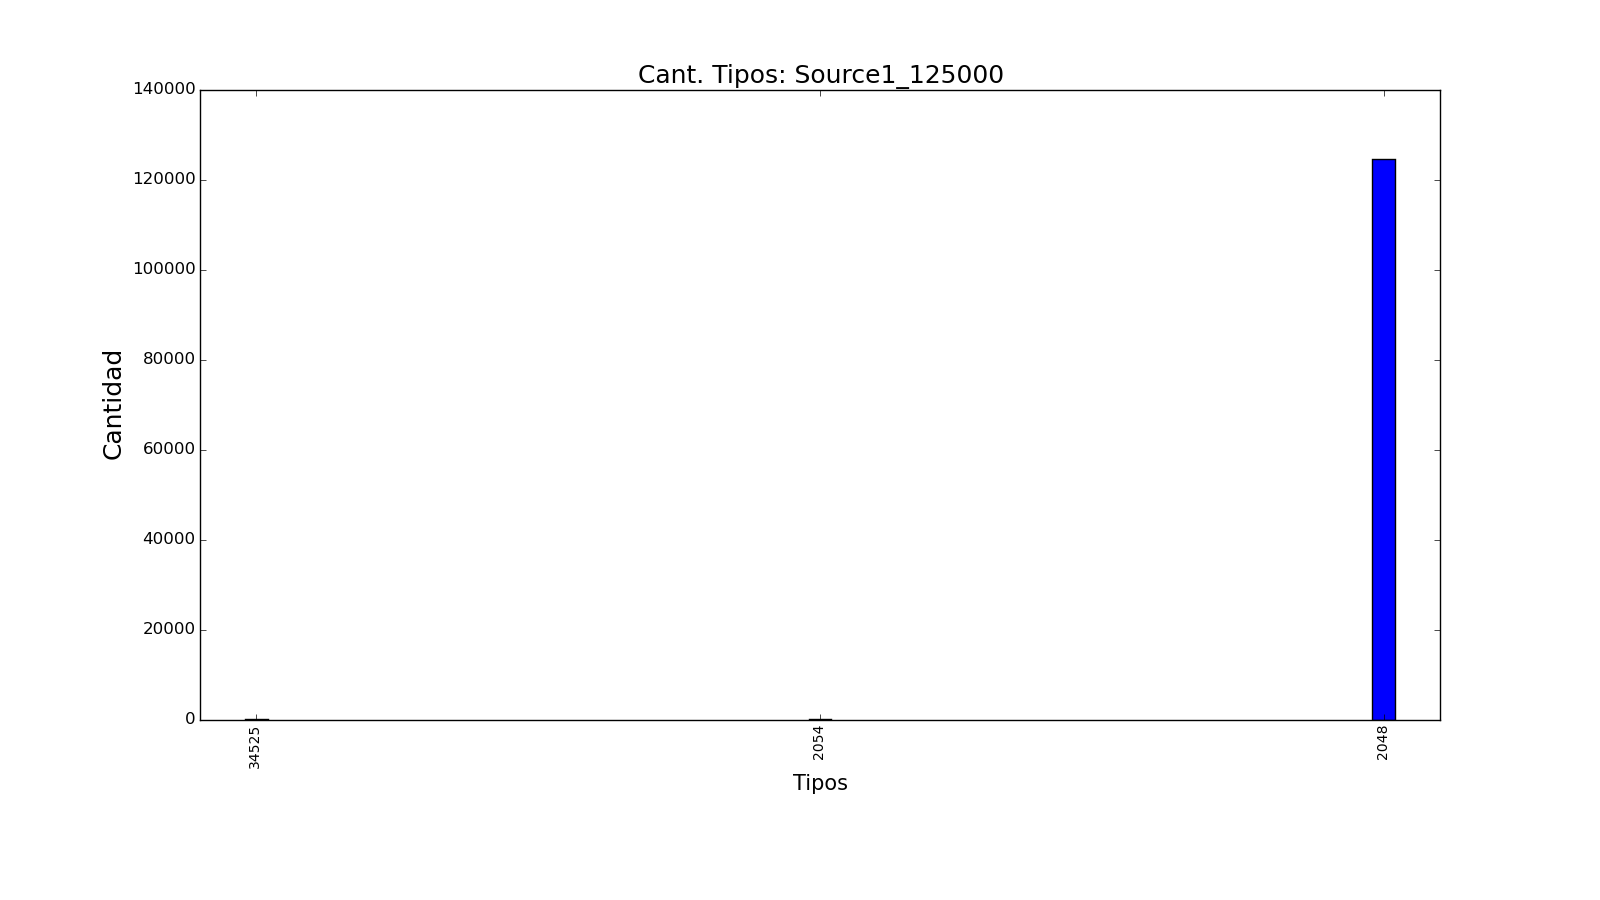
\includegraphics[width=1\textwidth]{../resultados/Casa/histogram_types.png}
       \caption{Protocolos de los paquetes capturados}
       \label{red-hogarena-types}
\end{figure}

\begin{figure}[H]
       \centering
       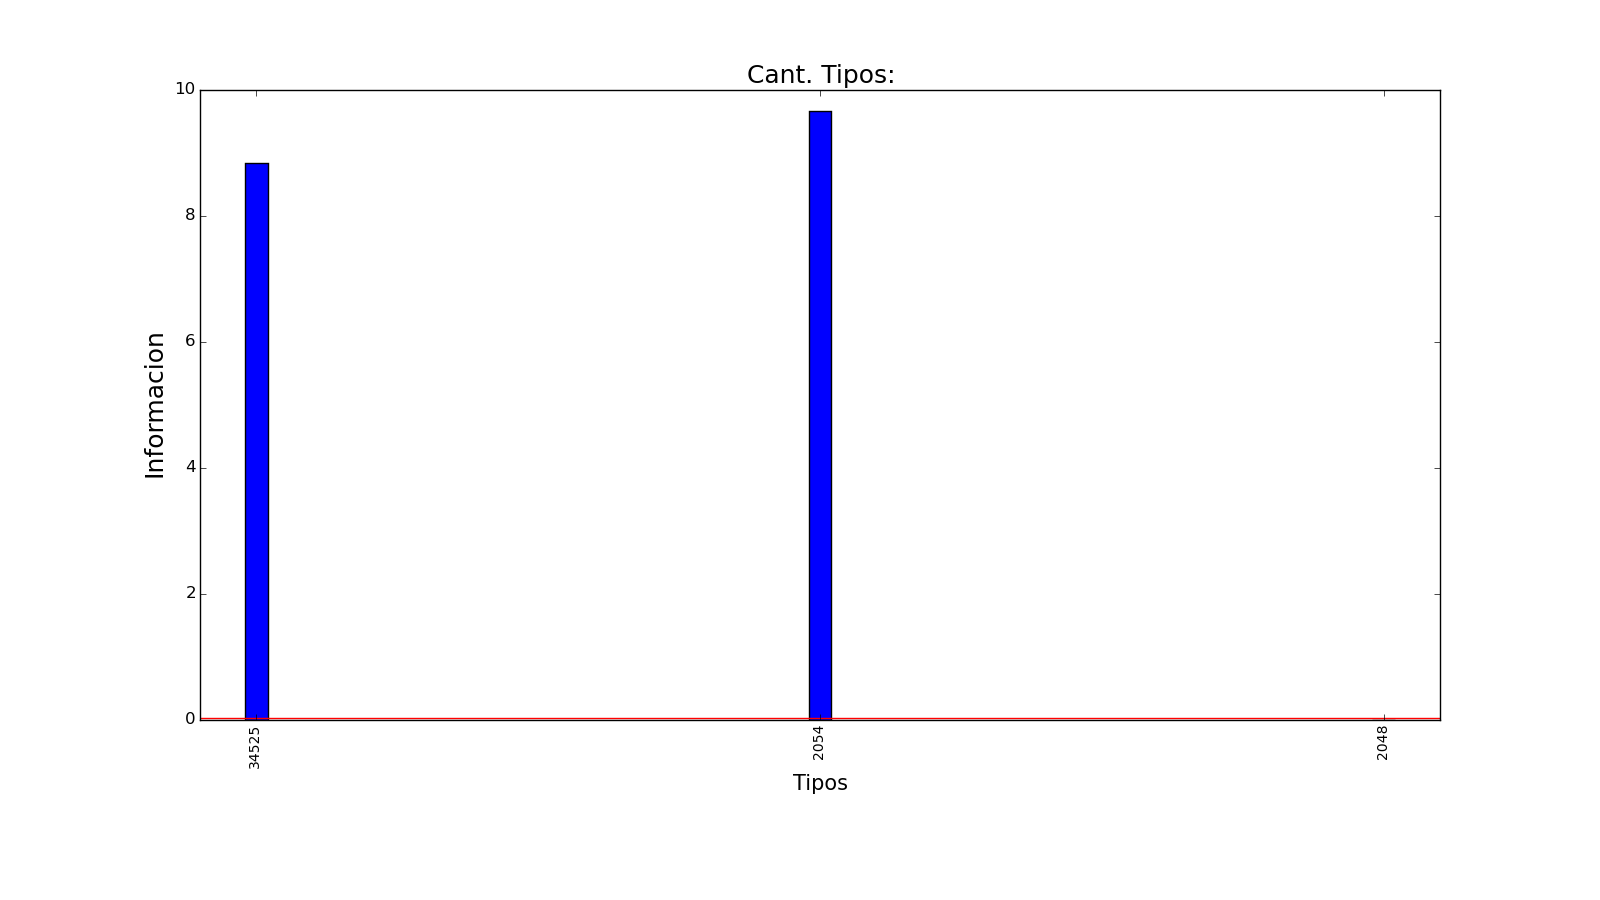
\includegraphics[width=1\textwidth]{../resultados/Casa/histogram_types_information.png}
       \caption{Información de los protocolos de los paquetes capturados}
       \label{red-hogarena-types-info}
\end{figure}

Como podemos observar, de acuerdo a la definición de protocolo distinguido que dimos anteriormente, el protocolo IPv4 sería el único distinguido en esta fuente. Esto resulta razonable, ya que la cantidad de paquetes IPv4 es mucho mayor que la cantidad de paquetes IPv6 y ARP. La información de los paquetes IPv4 es \textbf{0.00491352086592}, mientras que la entropía de la fuente es \textbf{0.0359827861687}. Se observa claramente como la información es menor a la entropía.


\begin{figure}[H]
       \centering
       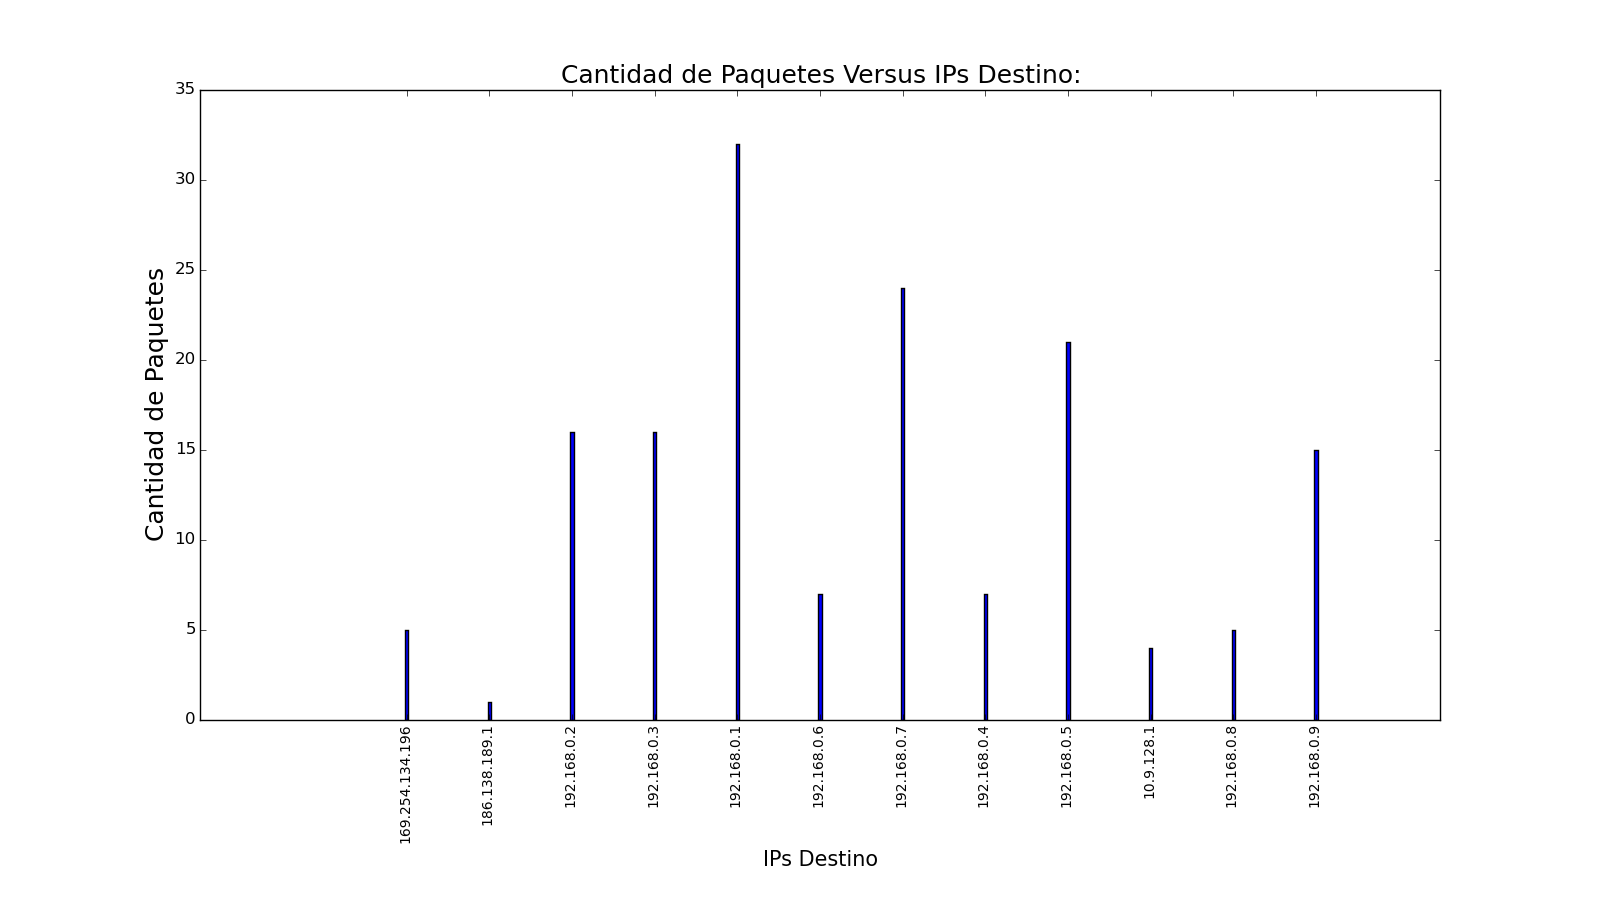
\includegraphics[width=1\textwidth]{../resultados/Casa/histogram_dst.png}
       \caption{IPs destino de los paquetes ARP}
       \label{red-hogarena-arp-destination}
\end{figure}

\begin{figure}[H]
       \centering
       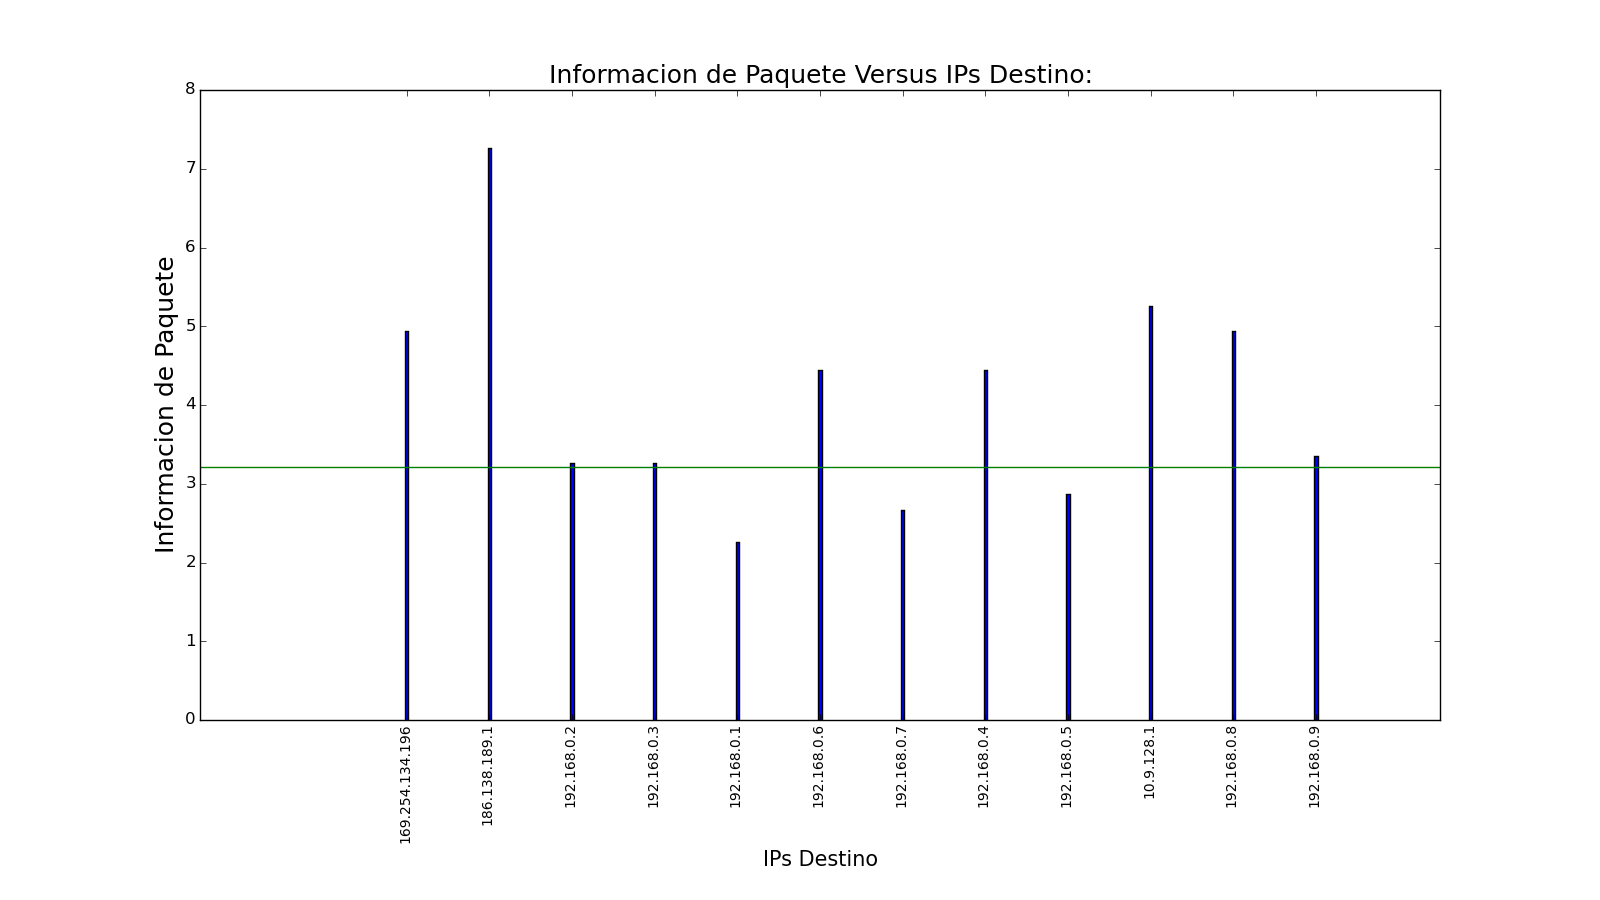
\includegraphics[width=1\textwidth]{../resultados/Casa/histogram_dst_information.png}
       \caption{Información de IPs destino de los paquetes ARP}
       \label{red-hogarena-arp-destination-info}
\end{figure}

En este caso el valor de la entropía es de \textbf{COMPLETAR}, y se pueden observar tres IPs que se encuentran debajo de este valor, por lo que consideramos que son nodos distinguidos en la red. Dichas IPs son:
\begin{itemize}
\item IP: \textit{192.168.0.1} con valor de información de \textbf{COMPLETAR}
\item IP: \textit{192.168.0.7} con valor de información de \textbf{COMPLETAR}
\item IP: \textit{192.168.0.5} con valor de información de \textbf{COMPLETAR}
\end{itemize}

A continuación se muestra el tráfico de la red para poder reconocer con qué dispositivos se condicen los \textbf{nodos distinguidos}

\begin{figure}[H]
       \centering
       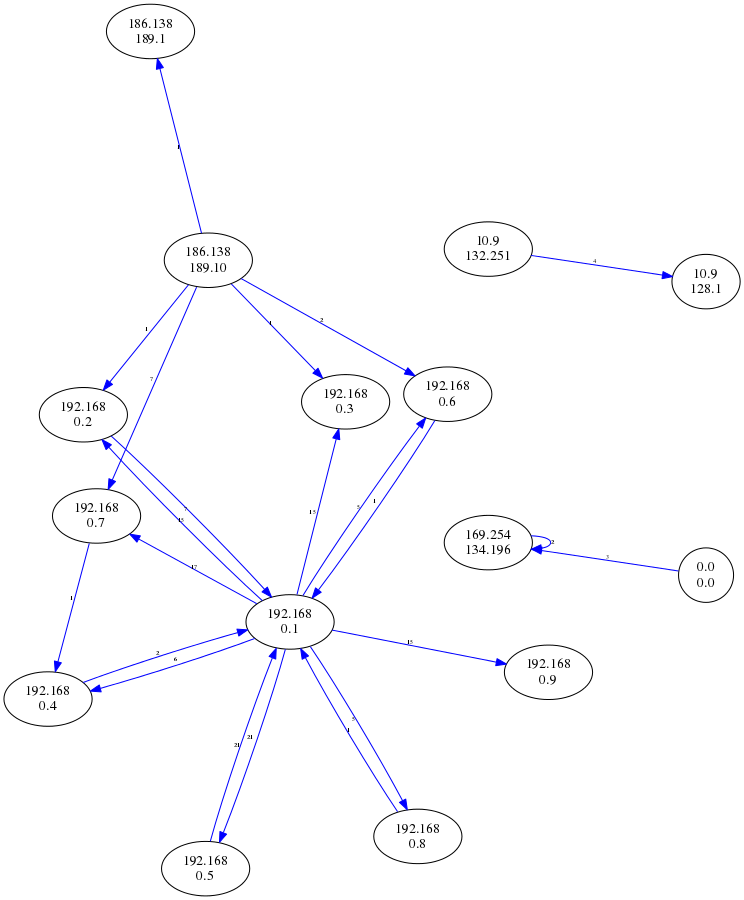
\includegraphics[width=1\textwidth]{../resultados/Casa/network.png}
       \caption{Tráfico de paquetes ARP}
       \label{red-hogarena-arp-traffic}
\end{figure}

Por un lado, se observa que gran cantidad de nodos se conectan al nodo con IP: \textit{192.168.0.1}, esto es asi ya que se trata del router.

Por otro lado, se observa un tráfico intenso (47 paquetes) del router al nodo con IP: \textit{192.168.0.7}, esto es así ya que esa IP se corresponde a una computadora de escritorio, que estaba realizando la descarga de un torrent, se puede notar como todo el tráfico se dirige del router a dicho nodo, pero no en sentido contrario.

Finalmente se ve un intercambio de paquetes importante entre el router y el nodo con IP: \textit{192.168.0.5}, en este caso se trata de una tablet que se encontraba navegando por distintas páginas de internet.
